\documentclass{article}
\usepackage{amssymb}
\usepackage{tkz-euclide}
\title{My Shool Geometry Notes}
\author{@mb6ockatf}
\date{\today}

\begin{document}
\maketitle
\tableofcontents
\section{Triangle: radius of inner circle}
$r = \frac{S_{ABC}}{0.5P}$
$$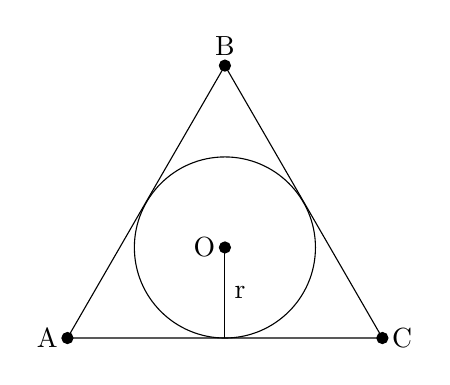
\begin{tikzpicture}
    \draw (0,0) -- (4,0) -- (2,3.46) -- cycle;
    \draw (2,1.15) circle (1.15);
    \filldraw[black] (2,1.15) circle (2pt) node[anchor=east]{O};
    \draw (2,1.15) -- (2,0);
    \filldraw[black] (2,0.575) circle (0pt) node[anchor=west]{r};
    \filldraw[black] (0,0) circle (2pt) node[anchor=east]{A};
    \filldraw[black] (2,3.46) circle (2pt) node[anchor=south]{B};
    \filldraw[black] (4,0) circle (2pt) node[anchor=west]{C};
\end{tikzpicture}$$

\end{document}
